\section{Experiments}
\label{sec:experiments}
We use Fetch push, reach and pick and place
tasks~\citep{plappert201802multigoalrl} in our experiments:
%
\begin{description}
  \item[Fetch-Reach] The tip of a robotic arm reaching a desired location.
  \item[Fetch-Push] A robotic arm pushing a block to a desired location.
  \item[Fetch-Slide] A robotic arm sliding a puck to a desired location.
\end{description}%
% 
\subsection{Baseline: Hindsight experience replay}
Hindsight Experience Replay~\cite{andrychowicz2016learning} targets
goal-conditioned tasks.
In goal-conditioned tasks, the rewards can be very sparse. Unless the agent hits
the goal, no value-able reward is learned and rest of the space is almost even
with respect to the rewards. To address this challenge, HER first assumes that
for every $\state_t$ the achieved goal $\goal_t = f_\goal(\state_t)$ is known.
Then HER simulates as if the achieved goal $\goal_t$ was the intended goal all
along by re-sampling the goal conditioned reward function.
More concretely, two time steps $t_1$ and $t_2 > t_1$ from the same episode in the replay memory are
sampled. The achieved goal at $t_2$ , $\goal_{t_2}$ is assumed to be the desired
goal at $t_1$ and the new simulated transition becomes $(\state_{t_1},
\act_{t_1}, \state_{t_1 + 1}, \Rew(\state_{t_1}, \goal_{t_2}, \act_{t_1}))$,
where $\Rew(\state_{t_1}, \goal_{t_2}, \act_{t_1})$ is the recomputed reward
instead of the observed reward $\Rew(\state_{t_1}, \goal^*_{e}, \act_{t_1})$ that
depends on the desired goal $\goal^*_{e}$ for that episode $e$.

HER can be applied to either DDPG or DQN, the experiments in
\citet{andrychowicz2016learning} show them to be applied on DDPG.

%
\begin{figure}%
  \def\frac{0.24}
  On Fetch Reach\\
  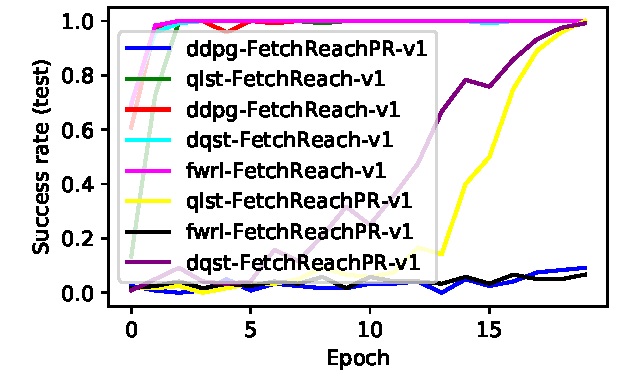
\includegraphics[width=\frac\columnwidth]{media/res/245b3c4-ce781a70-FetchReachPR-v1-fwrl-future-her_fwrl_path_reward/test/success_rate.pdf}%
  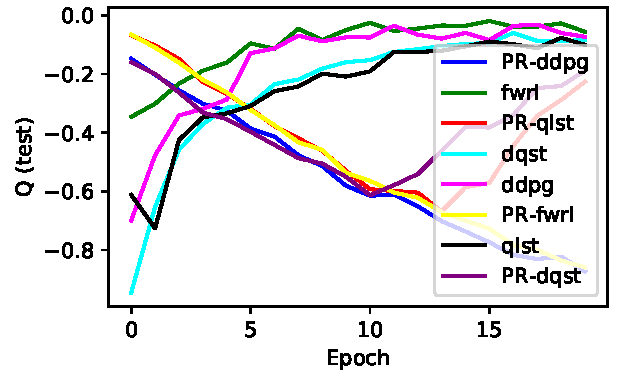
\includegraphics[width=\frac\columnwidth]{media/res/245b3c4-ce781a70-FetchReachPR-v1-fwrl-future-her_fwrl_path_reward/test/mean_Q.pdf}%
  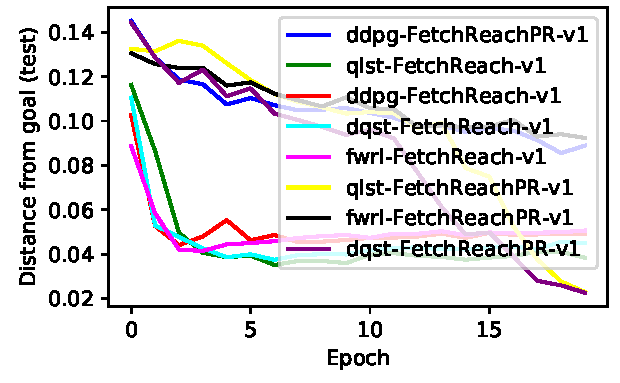
\includegraphics[width=\frac\columnwidth]{media/res/245b3c4-ce781a70-FetchReachPR-v1-fwrl-future-her_fwrl_path_reward/test/ag_g_dist.pdf}%
  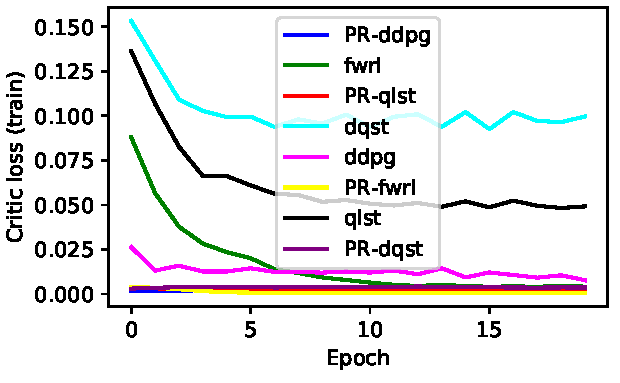
\includegraphics[width=\frac\columnwidth]{media/res/245b3c4-ce781a70-FetchReachPR-v1-fwrl-future-her_fwrl_path_reward/train/critic_loss.pdf}\\
  On Fetch Push\\
  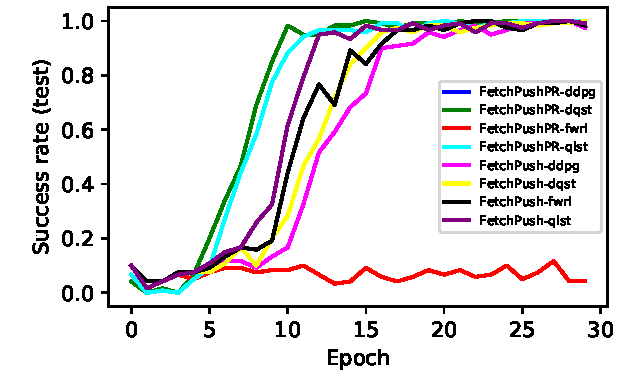
\includegraphics[width=\frac\columnwidth]{./media/res/be0910c-her_fwrl_path_reward-FetchPushPR-v1-fwrl/test/success_rate.pdf}%
  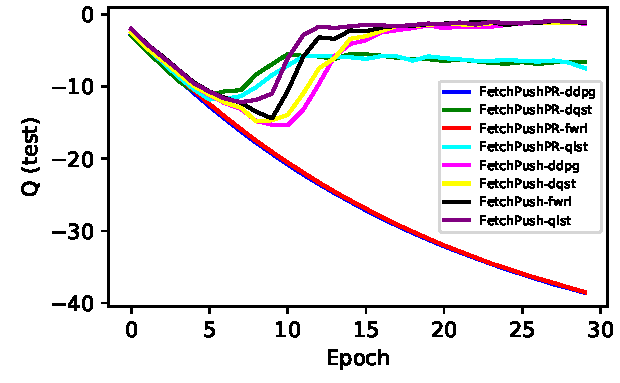
\includegraphics[width=\frac\columnwidth]{./media/res/be0910c-her_fwrl_path_reward-FetchPushPR-v1-fwrl/test/mean_Q.pdf}%
  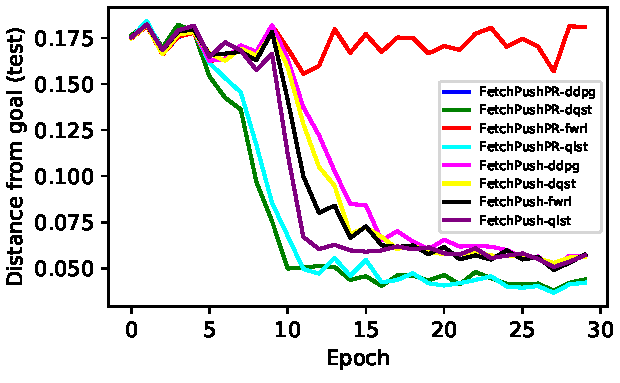
\includegraphics[width=\frac\columnwidth]{./media/res/be0910c-her_fwrl_path_reward-FetchPushPR-v1-fwrl/test/ag_g_dist.pdf}%
  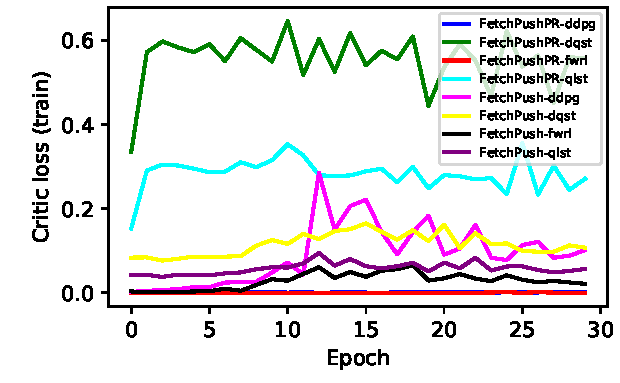
\includegraphics[width=\frac\columnwidth]{./media/res/be0910c-her_fwrl_path_reward-FetchPushPR-v1-fwrl/train/critic_loss.pdf}\\
  On Fetch Slide\\
  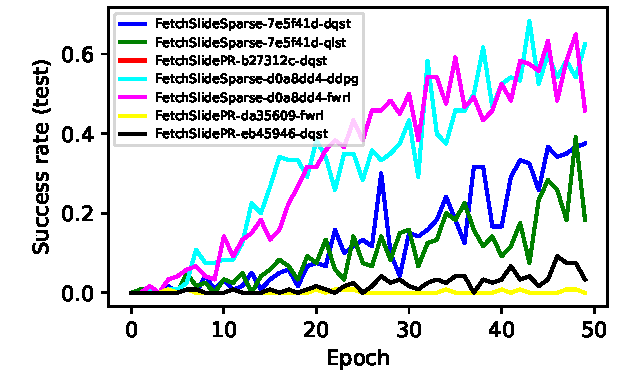
\includegraphics[width=\frac\columnwidth]{./media/res/eb45946-path_reward-FetchSlidePR-v1-dqst/test/success_rate.pdf}%
  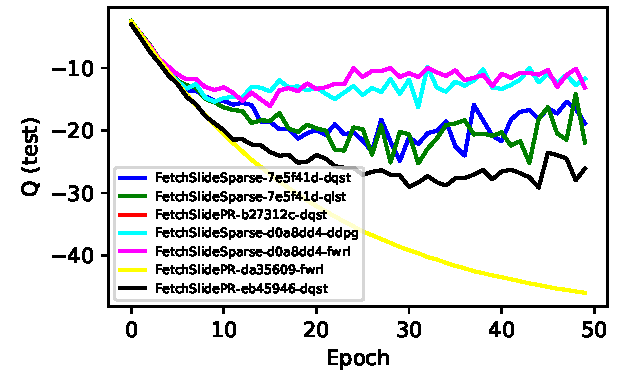
\includegraphics[width=\frac\columnwidth]{./media/res/eb45946-path_reward-FetchSlidePR-v1-dqst/test/mean_Q.pdf}%
  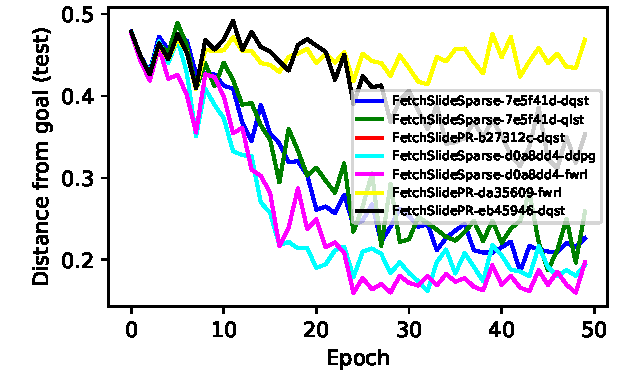
\includegraphics[width=\frac\columnwidth]{./media/res/eb45946-path_reward-FetchSlidePR-v1-dqst/test/ag_g_dist.pdf}%
  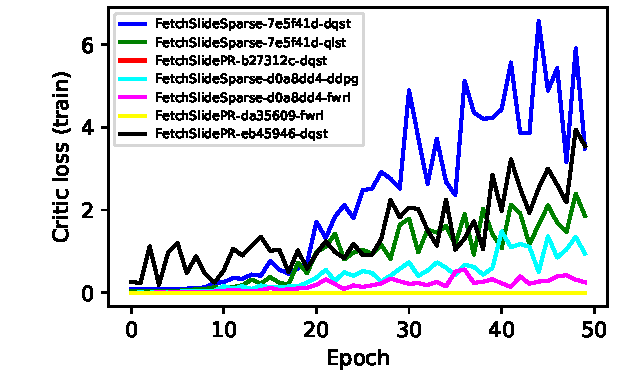
\includegraphics[width=\frac\columnwidth]{./media/res/eb45946-path_reward-FetchSlidePR-v1-dqst/train/critic_loss.pdf}\\
  On Fetch Pick And Place\\
  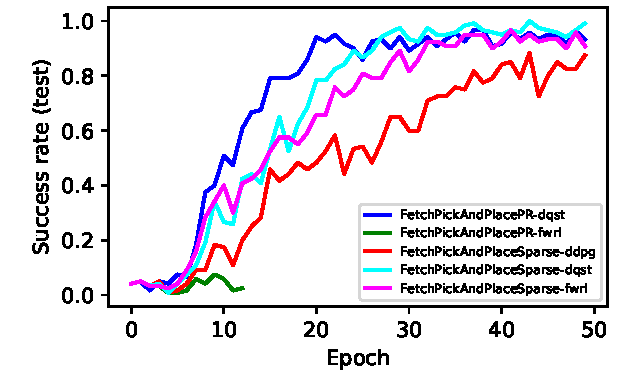
\includegraphics[width=\frac\columnwidth]{./media/res/d5cefef-path_reward-FetchPickAndPlacePR-v1-dqst/test/success_rate.pdf}%
  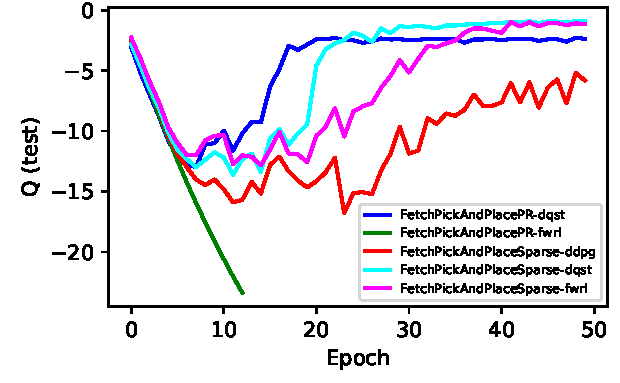
\includegraphics[width=\frac\columnwidth]{./media/res/d5cefef-path_reward-FetchPickAndPlacePR-v1-dqst/test/mean_Q.pdf}%
  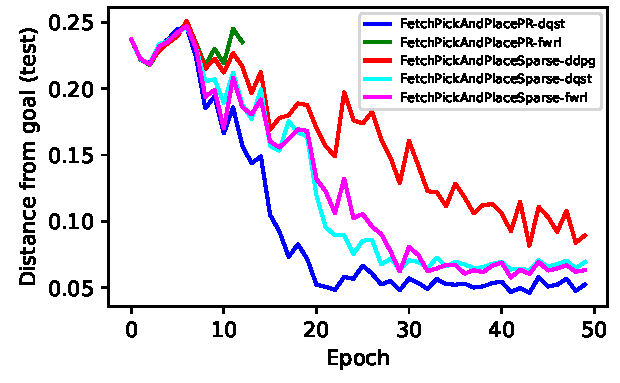
\includegraphics[width=\frac\columnwidth]{./media/res/d5cefef-path_reward-FetchPickAndPlacePR-v1-dqst/test/ag_g_dist.pdf}%
  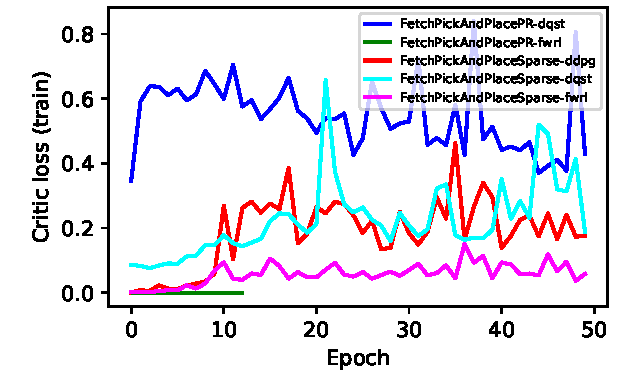
\includegraphics[width=\frac\columnwidth]{./media/res/d5cefef-path_reward-FetchPickAndPlacePR-v1-dqst/train/critic_loss.pdf}\\
  On Hand Reach \\
  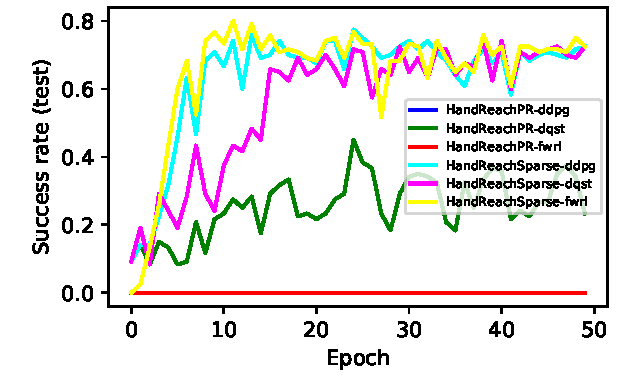
\includegraphics[width=\frac\columnwidth]{./media/res/d5cefef-path_reward-HandReachPR-v0-dqst/test/success_rate.pdf}%
  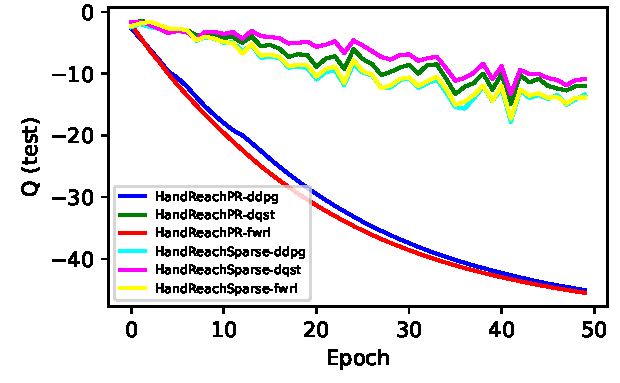
\includegraphics[width=\frac\columnwidth]{./media/res/d5cefef-path_reward-HandReachPR-v0-dqst/test/mean_Q.pdf}%
  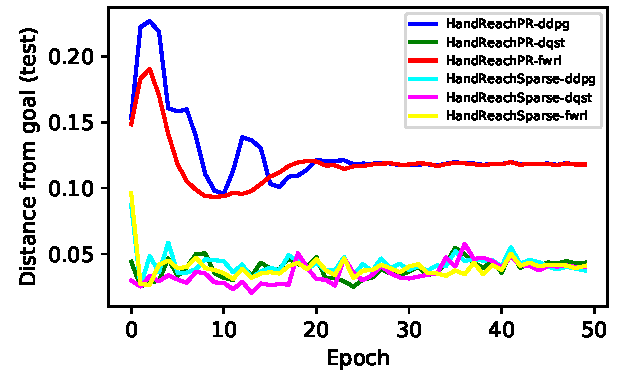
\includegraphics[width=\frac\columnwidth]{./media/res/d5cefef-path_reward-HandReachPR-v0-dqst/test/ag_g_dist.pdf}%
  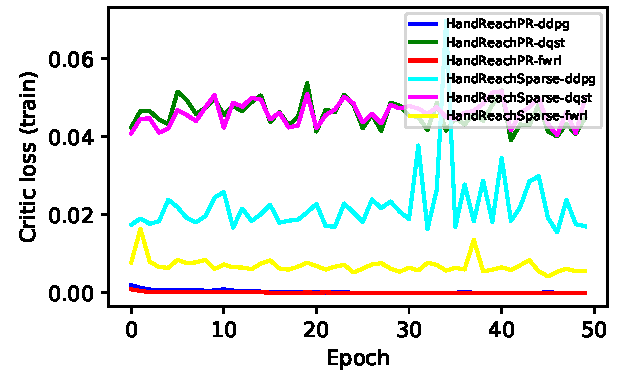
\includegraphics[width=\frac\columnwidth]{./media/res/d5cefef-path_reward-HandReachPR-v0-dqst/train/critic_loss.pdf}\\
  \label{fig:path-reward-1}%
  \caption{Effect of path reward on convergence in case of different loss
    functions on FetchReach. With path reward on PR-dqst
    ($\LossDDPG$ + $\LossStep$)
    and PR-qlst
    ($\LossDDPG$ + $\LossStep$ + $\LossLo$ + $\LossUp$), are able achieve high
    success rate and even that takes longer than usual. Out of the two PR-dqst
    does better. The terms with PR use path-rewards and hence less computation
    by avoid recomputation of reward function. It is interesting that PR-dqst
    and PR-qlst reach closer in terms of distance from goal probably because of
    absence of threshold.}%
\end{figure}%
% 